
\section{Issues and problems in WSN}
An important contribution of a wireless sensor network in the railway system is the availability of useful knowledge about energy consumption to the decision support systems.

Therefore, such acquisition systems are required to provide accurate data regardless of the quality of the acquisition sensors, \ac{EMI}, sensor supply fluctuations, among other error sources.

Through computational algorithms, the increase of communication reliability and fault tolerance is possible. Those computational algorithms detect outliers or, in the scope of this PhD, detect erroneous data that will disturb the outcomes of decision support systems. 



\subsection{Outlier and outlier detection}

\label{sec:def}
Outlier detection is a computational task to detect and retrieve information from erroneous data values. The definition is usually close to anomaly detection or deviation detection. 

Branch et al. (2006) identifies outlier detection as an essential step to either suppress or amplify outliers and precedes most data analysis routine, \cite{class:branch:2006}. Abid et al. (2016) points the need of detecting aberrant data and sensors within an \ac{WSN}, \cite{nn:abid:2016}.  Zhuang and Chen (2006) extends the outlier definition to the case where the outliers are introduced in sensing queries and in sensing data analysis, \cite{nn:zhuang:2006}.

%%%%%%%%%%%  outlier defnition in the scope of my phd
\vspace{1em}

In the scope of the PhD, an outlier is a data value or a data instance that do not represent the correct consumption status.

The threshold of what is an outlier or not (or a value that do represent the correct consumption status or not) is given by the output of the subsystem that is immediately after the acquisition of consumption status subsystem, the decision support subsystem, gave a correct output or not. Figure \ref{fig:general} illustrates the integration of the consumption acquisition subsystems with the decision support subsystem.


\begin{figure}[h!]
	\centering
	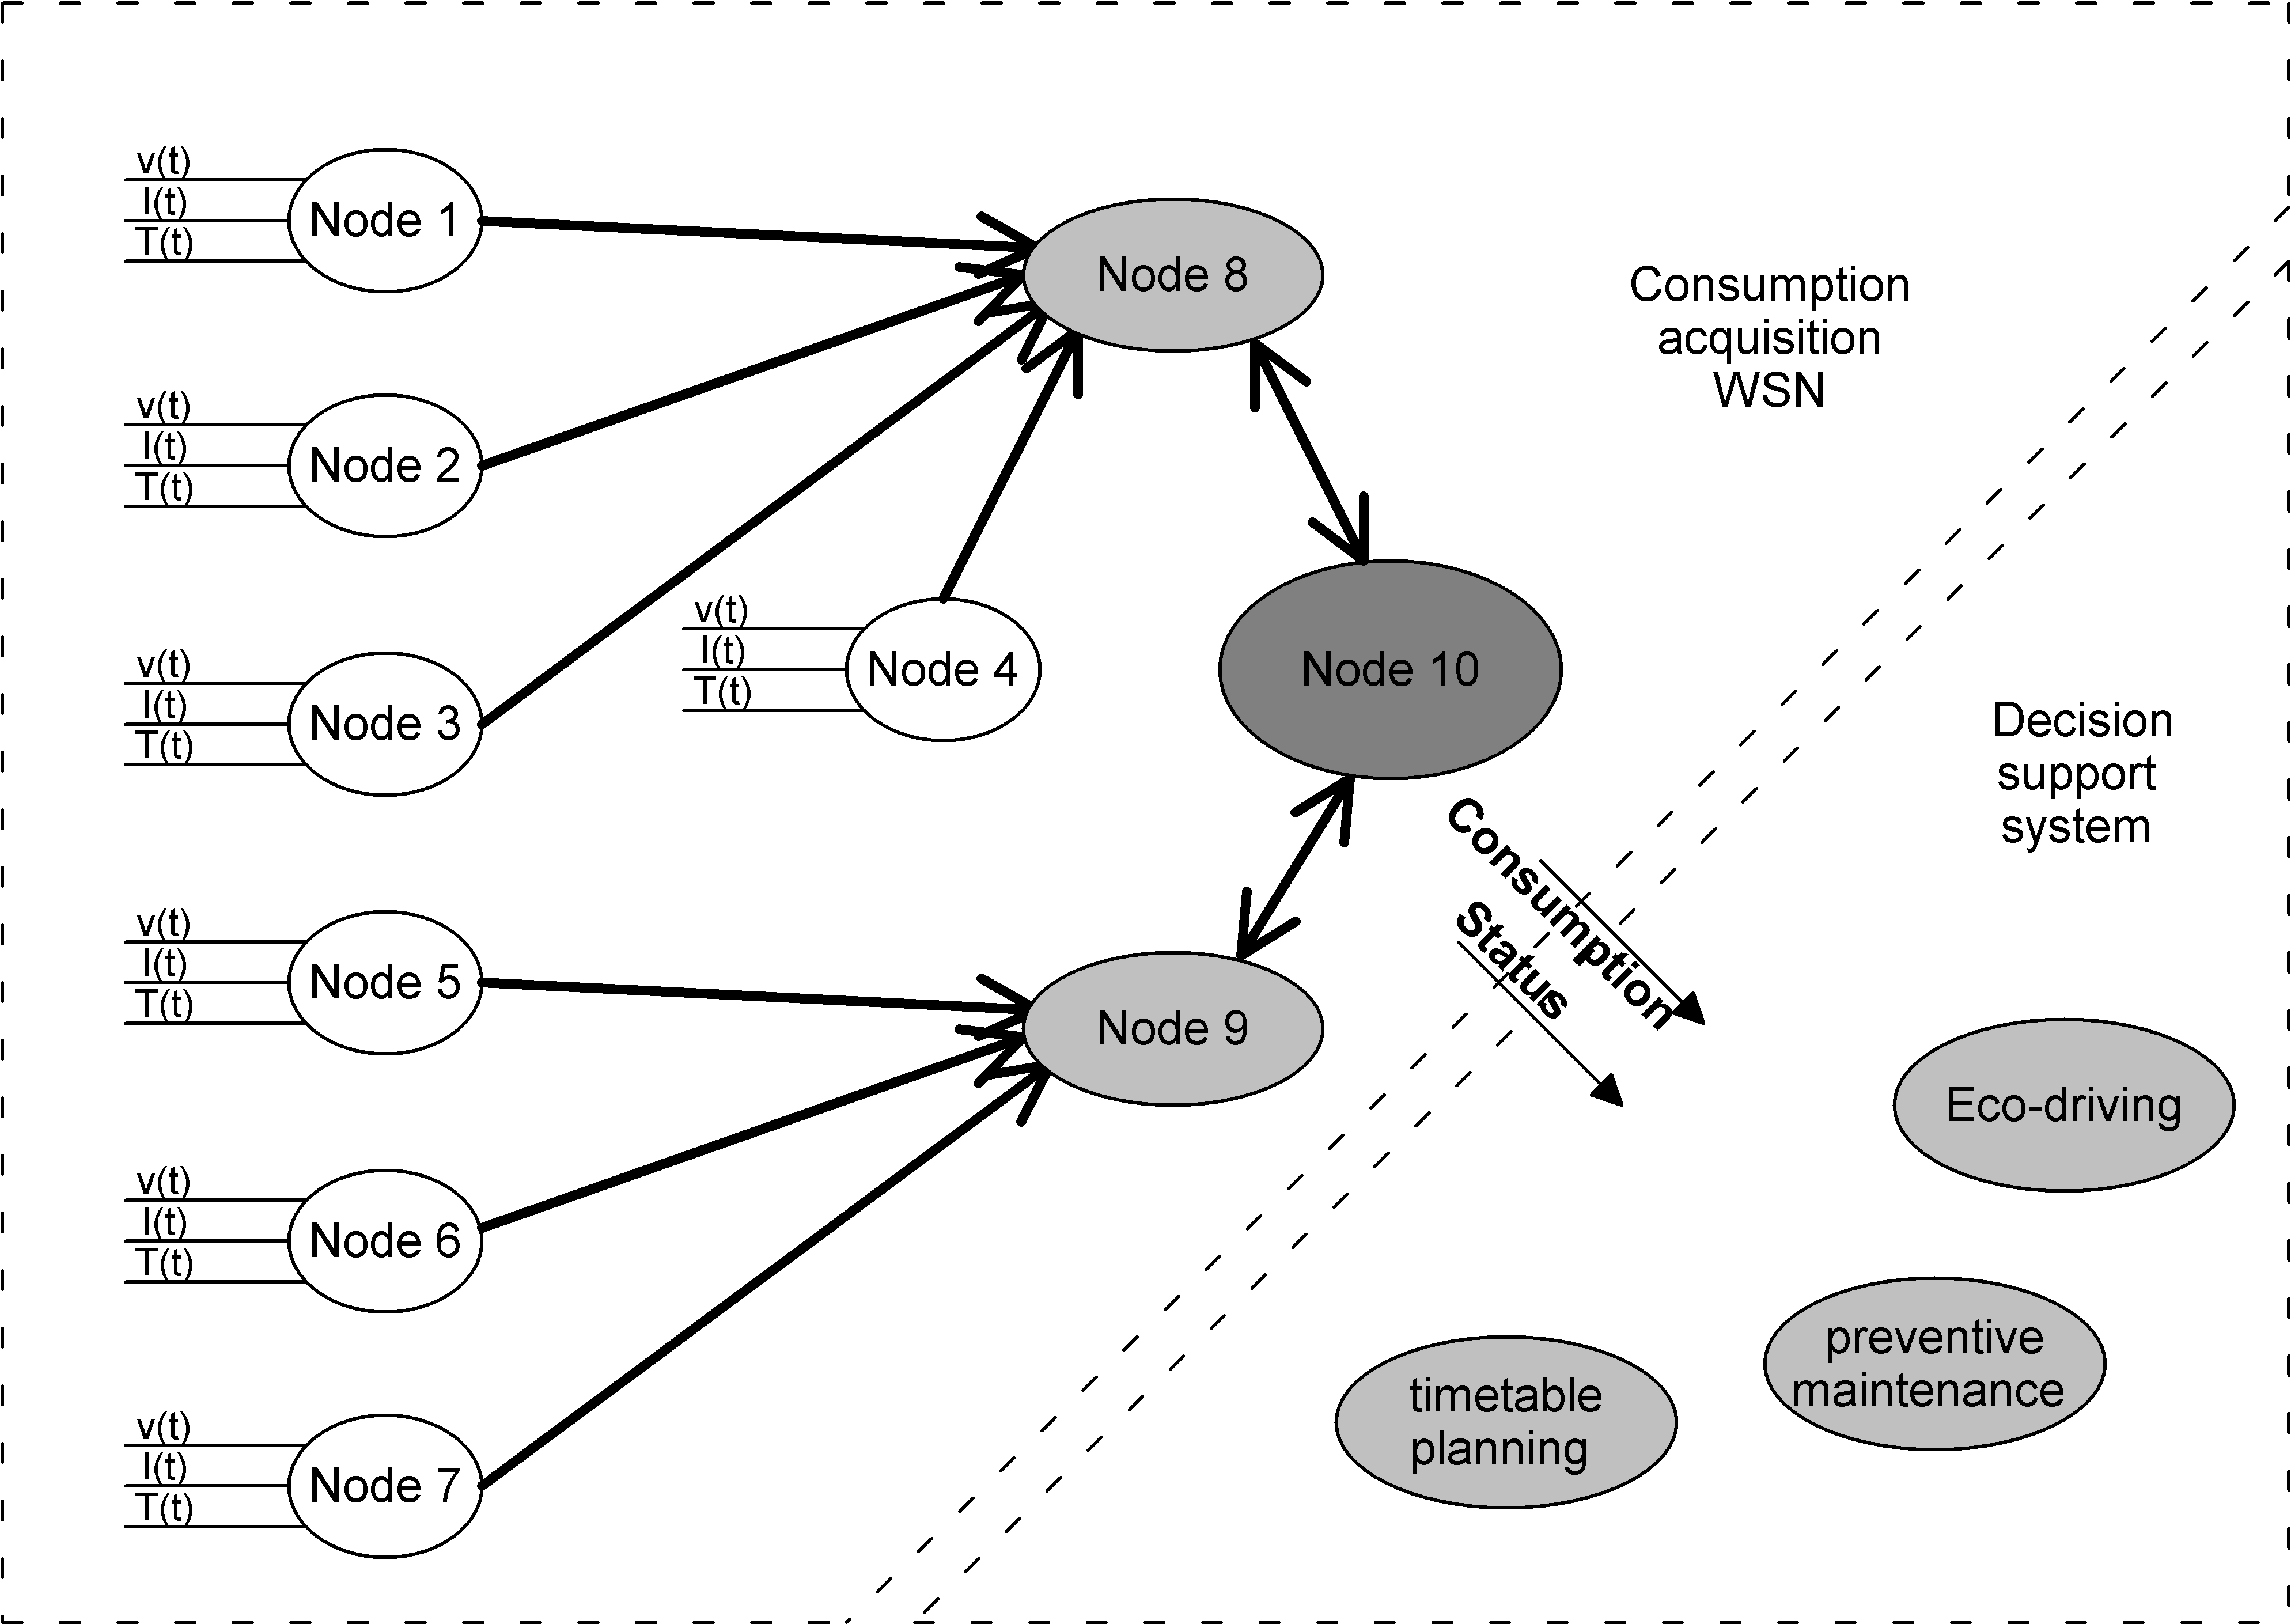
\includegraphics[width=0.7\textwidth,keepaspectratio]{figures/36.Outlier/general}
	\caption{Integration of the \ac{WSN} with a decision support system. }
	\label{fig:general}
\end{figure}

%\newpage
Without an outlier detection mechanism, the decision support subsystem may have the following outputs:


\begin{description}
	\setlength\itemsep{-0.5em}
	\item[Input deviation from real value lower than a threshold]
	The Decision Support Subsystem output is in accordance to the real consumption conditions.
	\item[Input deviation from real value greater than a threshold]
	The Decision Support Subsystem output is not in accordance to the real consumption conditions.	
\end{description}

The problem of taking decisions based on wrong considerations of the consumption status is that it may lead to loss in desirable efficiency or increase of costs.

Let us consider a simple and hypothetical example where the \ac{DSS} will provide an output towards suggesting an action in preventive maintenance based on the usage of a component. Considering that the usage of the component is depending on the counting of situations that the component is working above the nominal conditions. Without an outlier detection mechanism, the outliers will induce the \ac{DSS} in counting situations of overcharge of the component, where the measurement is not related to working nominal conditions but is related to external influences, such as \ac{EMI} or temperature. The output of \ac{DSS} may suggest a preventive maintenance on a component that is working in proper conditions.

To conclude, with an outlier detection mechanism in the consumption acquisition subsystem the decision support subsystem may know if the value of consumption is an outlier or not and, with that information, the \ac{DSS} output will be more accurate with the real conditions of operation.


\subsection{Literature review of Outlier detection in \ac{WSN}}
\label{sec:od_wsn}
\ac{WSN} has been widely used in several applications in several domains such as industrial, scientific, medical and others. Those applications have been supported by the advances in wireless technologies as well as in the evolution of microcontroller technologies, with enhanced processing capabilities associated with reduced energy consumption.

\subsubsection{Motivation}

Rajasegarar et al. (2007) points an important motivation for the inclusion of computational algorithms, i.e. outlier detection algorithms, to reduce the transmission of erroneous data, since in WSNs, the majority of the energy consumption occurs in radio communication, \cite{class:rajasegarar:2007}. In particular, they present the case of Sensoria sensors and Berkeley motes, where the energy consumption in communication exceeds, in ranges from 1000 to 10000, the energy consumption of computation.

Thus, this raises a research opportunity to reduce the communication usage of $\mu C$s, by adding processing features, where the small increase in the computation will significantly reduce the energy consumption in the transmission. These processing features are, among others, the outlier detection algorithms.


On the field of the quality of the data acquired by \ac{WSN}, the motivation of detecting outliers in data acquired from \ac{WSN} has been extensively presented in the literature. The need for acquire data from harsh or "highly dynamic" environments as well as the need to validate and extract knowledge from the acquired data are one of the main points in the motivation to study the outlier detection in \ac{WSN},  \cite{gen:zhang:2010,gen:chandola:2009,stat:ghorbel:2015,class:martins:2015b}.



\subsubsection{Research areas}
Zhang et al. identifies the outlier detection research areas in three domains, \cite{gen:zhang:2010} : 

\begin{itemize}
	\item Intrusion detection: Situation caused by malicious attacks, where the detection techniques are query-driven techniques;
	
	\item Fault detection: Situation where the data suffer from noise and errors and where the detection techniques are data-driven ones;
	
	\item Event detection: Situation caused by the occurrence of one atomic or multiple events and where the majority of the research has been developed due to its complexity.
\end{itemize}

Based on the division of this three domains, the upcoming research is intended to be focused on the event detection and fault detection techniques. Specifically, the main goal for this research will be the event detection algorithms.


\subsubsection{Challenges}

The challenges of outlier detection in WSNs are related to the quality of the acquisition of the sensors, the reliability of the modules in terms of energy or environmental susceptibility, and the communication requirements and restrictions.

Zhang et al. lists the challenges as the following,  \cite{gen:zhang:2010}:

\begin{itemize}
	\setlength\itemsep{-0.5em}
	
	\item Resource constraints;
	
	\item High communication costs;
	
	\item Distributed streaming data;
	
	\item Dynamic network topology, \\ frequent communication failures, \\ mobility and heterogeneity of nodes;
	
	\item Large-scale deployment;
	
	\item Identifier outlier sources;
	
\end{itemize}

Branch et al. (2006)  identifies an important challenge, where the probability of occurrence of outlier events are extremely small, \cite{class:branch:2006}. Other authors identify the large amount of data as the main challenge for outlier detection in WSN, \cite{nn:abid:2016, stat:sheng:2007}. In addition, some studies highlights the inexpensive and low fidelity sensors as the main reason for the error generation and the main challenge is identified on the distributed streaming data among a large amount of sensors, \cite{nn:zhuang:2006}. Another challenge is pointed to be  the processing of data from sensors that generate continuously data, that is uncertain and unreliable, \cite{stat:ghorbel:2015}. 

To conclude, the main challenge will be the usage of inexpensive and low fidelity sensors that will be affected by the rush railway environment. Complementary, the main challenge of using outlier detection mechanisms in the railway \ac{WSN} is the balance between the detection accuracy and the influence that undetected data-instances will induce in other subsystems (in particular in decision support systems dependent on data from the \ac{WSN}). In addition, the detection accuracy is directly related with the memory usage, computational requirements, communication overhead, etc. 


\subsection{Taxonomy of Outlier Detection Techniques}
\label{sec:taxon}
The study of detection techniques requires a well-defined taxonomy framework that addresses the related work on the different areas. 
This taxonomy is well defined and solid in the literature, where the works of Zhang et al. (2010) and Chandola et al. (2009) reflect a similar approach on presenting a taxonomy for outlier detection techniques, \cite{gen:zhang:2010, gen:chandola:2009}.

In the following sections, a coverage in relevant techniques is presented:

\begin{itemize}
	\setlength\itemsep{-0.5em}
	\item Classification based techniques.
	\subitem Bayesian Networks
	\subitem Rule-based techniques
	\subitem Support Vector Machines
	
	\item Statistical based techniques.
	\subitem Parametric --- Gaussian based
	\subitem Non-parametric --- Histogram based
	\subitem Non-parametric --- Kernel function based
	
	\item Nearest Neighbor-based techniques.
	\subitem Using distance
	\subitem Using relative density
	
	\item Clustering based techniques.
	
	\item Spectral Decomposition based techniques.
	
\end{itemize}

\begin{comment}


\subsection{Classification based techniques}
\label{sec:classbased}

Classification based techniques are based on systematic learning approaches which use sets of data. 
The supervised approaches require previous knowledge to train a model (or classifier) from a set of data instances (or training data) and classifies a new data instance as normal or as outlier. 
The unsupervised approaches do not require knowledge and learn the boundary around normal instances, declaring the new instance as normal or as outlier depending if the data instance is outside of the boundary of the previous data sets.

The classification based techniques are listed as the following:

\begin{itemize}
	\setlength\itemsep{-0.5em}
	\item Neural Networks-based;
	\item Bayesian Networks-based;
	\item Rule-based;
	\item Support Vector Machines-based.
	
\end{itemize}

\vspace{0.5em}

Neural networks-based approaches are interesting strategies for outlier detection where a given neural network might be trained with only normal data-sets. 
At testing stage, the data instances that are similar to the training data-set are accepted by the neural network and then considered as normal. 
The remaining data-sets are rejected by the neural network due to their lack of similarity with normal data-sets. Thus, those data instances are considered as outliers. 
%Based on the table \ref{table:t3}, t
These techniques are classified as semi-supervised due to their need for normal data-sets for the training stage.

\vspace{0.5em}

Bayesian networks-based approaches are identified as prominent techniques for outlier detection in WSNs, being the reason why they are extensively covered further on in \ref{subsec:bay}.
Those techniques use probabilistic graphical models to detect outliers based on the interdependencies of different variables.

\vspace{0.5em}

Rule-based techniques, presented in \ref{subsec:rule}, classify an outlier based on a confidence value related to the number of the training instances correctly classified by a given rule and the total number of training instances covered by the same rule. For each test instance, all the rules are tested and the confidence value is ordered. The output of this outlier detection technique is given by the inverse of the confidence value of the rule that better captures the test instance.

\vspace{0.5em}

Support Vector Machine (SVM) techniques are used for outlier detection to classify a given instance based on the fitness of a hyper-sphere to the data in a higher dimensional space. 
The hyper-sphere is obtained with a linear optimization algorithm where the objective function of this linear optimization problem is to minimize the radius R that cover the majority of the image vectors. The output of the SVM applied to OD is the classification of the image vectors as outliers if they are outside of the hyper-sphere. The SVM techniques are presented in \ref{subsec:svm}.
\subsubsection{Bayesian Networks}
\label{subsec:bay}
\cite{gen:zhang:2010} divide the bayesian network based techniques in three categories: 

\begin{itemize}
	\setlength\itemsep{-0.5em}
	\item Na\"{i}ve Bayesian Networks;
	\item Bayesian Belief Networks;
	\item Dynamic Bayesian Network Models;	
\end{itemize}

All those approaches use probabilistic graphical models to represent a set of variables and their probabilistic interdependencies. 
This graphical model aggregates the information from different variables and provides an estimate on the expectancy of an event to belong to the learned class.

\cite{class:xiang:2016} illustrates an application to measure the concentration of NO$_2$, CO and O$_3$ pollutants, using a bayesian network. All the three variables are all correlated and also depends on the temperature as presented in figure \ref{fig:xiang2016}. The real measurements acquired by the microcontroller are represented with (s) and the representations in (t) refers to the real concentration of those pollutants.

\begin{figure}[h!]
	\centering
	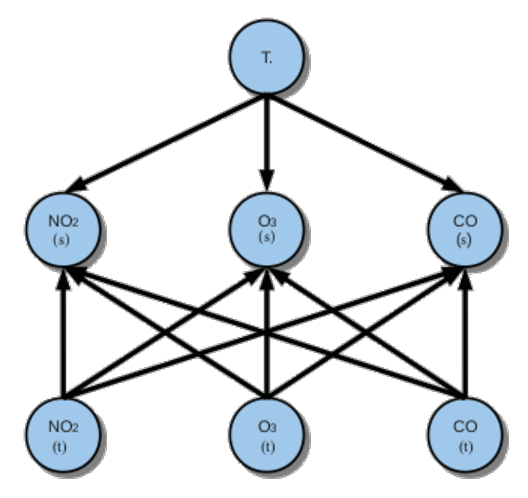
\includegraphics[width=0.60\textwidth,keepaspectratio]{figures/xiang2016}
	\caption{Application of a Bayesian Network to an atmospheric measurement system. }
	\label{fig:xiang2016}
\end{figure}

The three categories presented by \cite{gen:zhang:2010} differs between them where the first category captures the sensor nodes correlations on spatio-temporal domain; 
The second one considers not only the spatio-temporal correlations but also the conditional dependence of sensor attributes;
The third category proposes the measurement of state variables at a current time instance.

\cite{class:janakiram:2006} proposes the detection of outliers in sensor streamed data by capturing the conditional dependencies among the observation of it's attributes. this is made in three phases:

\begin{description}
	\setlength\itemsep{-0.5em}
	\item[Training Phase]  
	Phase where the Bayesian Belief Network is trained to capture the spatio-temporal correlations.
	\item[Testing Phase]  
	Phase where the trained BBN is tested on the level of accuracy and, if needed, the learned parameters are updated.
	\item[Inference Phase] 
	Phase where the missing values are inferred and the remaining streamed data are tested to detect if it is an outlier or not.
\end{description}

\cite{class:janakiram:2006} also defined the BBN, where the BBN is a directed graph, together with an associated set of probabilistic tables.
The graph is divided in nodes and arcs, where the nodes represents the variables and the arcs are the representation of the casual/influential relationship among variables.

The main contribution of BBN is the possibility to have a model that, with the dependency between uncertain variables (by filling a node probability table), it is possible to describe complex probabilistic reasoning about uncertainty.

\cite{class:janakiram:2006} describes their process in three steps:

\begin{itemize}
	%\setlength\itemsep{-0.5em}
	
	\item Constructing the Bayesian Belief Network
	\subitem \textbf{IF} a few variables have direct dependencies
	\subitem \textbf{AND} many of the variables are conditionally independent
	\subitem \textbf{THEN} all the probabilities can be computed from the joint probability distribution.
	
	\item Learning Bayesian Belief Networks
	\subitem \textbf{IF} the network structure is given
	\subitem \textbf{AND} all variables are fully observable in the training examples
	\subitem \textbf{THEN} estimating the conditional probabilities is enough
	\subitem
	\subitem \textbf{IF} the network structure is given
	\subitem \textbf{AND} some of the variables are observable
	\subitem \textbf{THEN} apply neural network using Gradient Ascent Procedure
	\subitem
	\subitem \textbf{IF} the network structure is unknown
	\subitem \textbf{THEN} Use heuristic search
	\subitem \textbf{OR} Use constraint-based technique to search through potential structures
	
	
	\item Inferring from Bayesian Belief Networks
	\subitem \textbf{THESIS} The probability distribution of certain attributes might be inferred
	\subitem \textbf{PROOF} Given the fact that the values that other attributes can take are known	
\end{itemize}

\cite{class:paola:2015} proposes an adaptive distributed Bayesian approach for detecting outliers in data collected by a WSN.
The focus of the proposed algorithm is the optimization of outlier classification accuracy, time and communication complexity and also considering externally imposed constraints on conflicting goals. The proposed algorithm is intended to run in each sensor node. 

From the individual sensor node point of view, this algorithm consists in two phases:

\begin{description}
	\setlength\itemsep{-0.5em}
	\item[Outlier detection]  
	Where, based on sensor readings and on the collaboration with neighbors, is made the probabilistic inference where the results are evaluated in three metrics: classification accuracy, time complexity and communication complexity.
	
	\item[Neighborhood selection] 
	Where the best neighbors are identified and selected to cooperate with, and, in addiction, to correspond to a reconfiguration of the Bayesian Network structure.
\end{description}

In the global point of view, if there is a high number of cooperating nodes, the classification is naturally higher with the drawback if increasing the processing time and communication complexity (thus resulting in increased detection delay and increase of energy consumption).

\cite{class:xiang:2016} proposes the addition of recover and recalibrate the drifted sensors simultaneously based on the usage of a Bayesian network. 
The authors have applied their algorithm to the measurement of the variables in the sensor readings of the NO$_2$, CO and O$_3$ pollutants, as previously presented in figure \ref{fig:xiang2016}.
Based on the correlations of the sensor readings and on the temperature influence, the algorithm itself detects the outliers, recover valid information and adjust the BBN to automatically recalibrate the sensor.




\subsubsection{Rule-based techniques}
\label{subsec:rule}
Rule based is another classification based technique for outlier detection. Similarly, this technique is based on a training stage from a data-set and a model generation to detect new data-instances based on history values.

Rule based techniques depends on two steps \cite{gen:chandola:2009}:

\begin{itemize}
	%\setlength\itemsep{-0.5em}
	\item \textbf{1. Learn rules from the training data-set}\\
	Using a learning algorithm (i.e. RIPPER, Decision Tree, etc.)\\
	Where each rule has an associated confidence value 	proportional to the ratio:\\
	{\centering	$\text{\footnotesize Confidence Value} = \frac{\text{number of training instances correctly classified by the rule}}{\text{number of total training instances covered by the rule}}$
	}
	
	\item \textbf{2. Find for each test instance the rule}\\
	That better capture the given test instance.
	
	\item \textbf{$\Rightarrow$ The anomaly score is}\\
	The inverse of the confidence value for the rule that better capture the test instance.
	
\end{itemize}

\cite{class:islam:2016} proposes an algorithm for outlier detection inserted in rule-based taxonomy. They propose a new belief-rule-based association rule, with the focus on handling various types of uncertainties. 

Due to the nature of the sensor data, a traditional inference mechanism cannot be used. Therefore, they propose a new inference mechanism for the rule-based algorithm that consists of an input transaction database that is converted into the following:
\begin{itemize}
	\setlength\itemsep{-0.5em}
	\item belief transaction database;
	\item support calculation;
	\item belief matrix;
	\item confidence calculation;
	\item belief association rule discovery.
	
\end{itemize}


%\newpage
\vspace{1.5em}

\subsubsection{Support Vector Machines}
\label{subsec:svm}
Rather than performing outlier detection in the central node, \cite{class:rajasegarar:2007} proposes a 
distributed approach to:

\begin{itemize}
	\setlength\itemsep{-0.5em}
	\item performs detection on local data at each node
	\item and communicates to the parent node only the summary information to perform at upper layer the global classification of the data.	
\end{itemize}

Their proposal is based on a one-class quarter sphere SVM and is divided into 2 parts:

\begin{itemize}
	\setlength\itemsep{-0.5em}
	\item \textbf{Anomaly detection  algorithm}
	\subitem The OD is supported by previous works where, with the fitness approach of a hypersphere to the data in a higher dimensional space, and by applying a linear optimization to the problem of fitting the hypersphere with minimal radius R, having the center fixed at the origin and encompassing the majority of the image vectors.
	\subitem The result of the linear optimization problem is the classification of the image vectors as:
	
	\vspace{-1em}
	
	\subitem  \textbf{$\rightarrow$ Support Vectors}, if inside the sphere;
	\subitem  \textbf{$\rightarrow$ Outliers}, otherwise.
	\vspace{1em}
	
	\item \textbf{Distributed anomaly detection}
	\subitem \textbf{1$^{st}$ step:} Each sensor node runs the entire AD algorithm on local data;
	\subitem \textbf{2$^{nd}$ step:} The resulting radius is sent to the parent node;
	\subitem \textbf{3$^{rd}$ step:} Each parent computes the global radius;
	\subitem \textbf{4$^{th}$ step:} Parents sends the radius to children nodes;
	\subitem \textbf{5$^{th}$ step:} Children compares global radius with local one and updates parameters.
	
\end{itemize}


\cite{class:xu:2012} proposes a KNN-SVM which is a Support Vector Machine based on K-Nearest Neighbor Algorithm.

Despite KNN taxonomy is presented further on in \ref{sec:nnbased}, in a synthesis  the KNN is a distance-based approach that detect outliers in data-instances lying in the sparsest regions or lying in the outside of a given model boundary of the feature space.

Considering the Quarter sphere SVM technique proposed by \cite{class:rajasegarar:2007} the KNN-SVM combine the origin and the radius R that contain most of the samples and introduces kernel functions to make the optimization region more tighten. 

\subsection{Statistical based techniques}
\label{sec:statbased}



\cite{gen:chandola:2009} identifies the statistical techniques for anomaly detection based on the assumption that, in a stochastic model, the most common data instances occur in high probability regions and the anomalies occur in low probability regions.

To detect anomalies, parametric techniques are suggested, since those techniques \textbf{assume} the knowledge of the underlying distribution and \textbf{estimate} the parameters from a given data set. Non-parametric techniques differ from parametric ones without the need of assuming the knowledge of the distribution.

\cite{cluster:andrade2016} lists some statistical parametric techniques: 

\begin{description}
	\setlength\itemsep{-0.5em}
	\item[Peirce's Criterion]  
	This statistical parametric method is based on a normal distribution.
	\item[Chauvenet's Criterion]  
	Is based on the assumption that a given arbitrary measurement may be rejected, if the probability of having the deviation for the average value is lower than the inverse of the double of the number of measurements. 
	
\end{description}

\subsubsection{Parametric --- Gaussian based}
\cite{gen:zhang:2010} summarizes parametric techniques as an anomaly detection strategy based on the following steps:

\begin{itemize}
	\setlength\itemsep{-0.5em}
	\item The available knowledge is generated from a known distribution;
	\item The distribution parameters is then estimated from the given data.	
\end{itemize}

The usage of Gaussian  models allows the spatial correlation of readings towards distinguishing between outlying sensors and event boundary. 

\subsubsection{Non-parametric --- Histogram based}
\cite{stat:sheng:2007} proposes a histogram-based method to reduce the communication cost on sensor networks. The main objective of this proposal is to collect hints (in a form of histogram) about the data distribution and, with the knowledge from these hints, unnecessary data is filtered and potential outliers are detected 


Complementary, \cite{stat:wang:2013} introduces clusters on incremental histogram scheme based on a divide and conquer strategy:

\begin{itemize}
	\setlength\itemsep{-0.5em}
	\item The wireless network is divided in clusters (based on adjacent nodes and data correlated strategy);
	\item The cluster head and cluster members updates the histogram incrementally and compares histograms in the form of Kullback-leibler divergence differentially (Kullback-leibler divergence is a convenient and robust
	method of measuring the difference between two data sets in a
	statistical sense.)
\end{itemize}

%%%%%%%%%%%%%%%
%%%%%%%%%%%%%%%
\subsubsection{Non-parametric --- Kernel function based}
\cite{gen:zhang:2010} synthesizes the concept of Kernel function non-parametric approaches as methods for estimating the probability distribution function for normal instances (and a new instance that occurs on a low probability area is declared an outlier). Later on in section \ref{sec:specbased} is presented the Kernel Principal Component Analysis (KPCA) used by \cite{stat:ghorbel:2014} for outlier detection in WSN's.

\cite{cluster:andrade2016} identify some kernel regression techniques: 

\begin{description}
	\setlength\itemsep{-0.5em}
	\item[Marzullo's Fault Tolerant Sensor Averaging (FTA) ] 
	Simple method for sensor fusion where the data assumed as anomalous is deleted.
	\item[Elmenreich's Confidence-Weighted Averaging (CWA) ] 
	The sensor's confidence are correlated with the sensor's variance.
	\item[CWA+FTA method ]
	This method combines both methods where the confidence-weighted average is calculated and two-thirds of the anomalous data is removed.
\end{description}


\subsection{Nearest Neighbor-based techniques}

\label{sec:nnbased}



A promissory technique is extensively explored in the literature with the concept of neighborhoods, based on the key assumption that normal instances occurs in dense neighborhoods and anomalies occurs far from their closest neighbors.





\subsubsection{Using distance}



\cite{class:branch:2006} proposes algorithms that implements nearest neighbor-based techniques for outlier detection in WSN's. The proposed unsupervised anomaly detection techniques use the following different algorithms:



\begin{itemize}
	
	\setlength\itemsep{-0.5em}
	
	\item The distance to the $k^{th}$ nearest neighbor;
	
	\item The average distance to the k nearest neighbors;
	
	\item the inverse of the number of neighbors, within a distance $\alpha$.	
	
\end{itemize}



\cite{nn:abid:2016} bases the detection technique on the distance between the current measurement and its neighbors. A synthetic database is generated based on the insertion of random values into a real database (in particular the Intel Berkeley lab WSN database).

The procedure is divided in two steps: 

\begin{itemize}
	
	\setlength\itemsep{-0.5em}
	
	\item \textbf{Step 1a)} For a given time-slot, the data values are sorted in a vector;
	
	\item \textbf{Step 1b)} After that, for a given point in the vector, Euclidean distance between the predecessor and successor is calculated and stored in a second vector;
	
	\item \textbf{Step 1c)} Based on the smallest distance between the current point and the predecessor or successor, the current point is linked;
	
	\item \textbf{Step 2} If the point in the vector is not linked (due to its distance between current point and predecessor/successor higher than a threshold), is declared an outlier;
	
\end{itemize}





\subsubsection{Using relative density}

\cite{gen:chandola:2009} defines the NN technique using relative density as a technique that estimates the density of the neighborhood of all data instances. Depending if the instance corresponds to a dense neighborhood or a low density one, the data is declared as outlier or normal.

\subsection{Clustering based techniques}
\label{sec:clustbased}
%\lipsum[4-4]

\cite{gen:chandola:2009} synthesizes the clustering techniques in three categories based on three different assumptions: 

\begin{itemize}
	
	\setlength\itemsep{-0.5em}
	
	\item The normal data instances are part of a cluster in the data and the outliers does not fit any cluster;
	
	\item The normal data instances are present close to its closest cluster centroid and the outliers lies far away from their closest cluster centroid;
	
	\item The normal data instances are part of large dense clusters and the outliers are part of small or sparse clusters.
	
\end{itemize}

\cite{clust:rajasegarar:2006} uses a technique to minimize the communication overhead by using clusters among the sensor readings. In a further step, it merges the clusters before the data is sent to other nodes.

\cite{cluster:andrade2016} presents a methodology to apply clustering and statistical techniques. The clusters are grouped according to the spatial position of the sensors and a k-means nearest-neighbor technique is used to provide a better understanding of the sensed environment. The proposed methodology follows a two-step procedure, starting with the usage of clustering information and followed by a statistical-based method. The statistical method is Elmenreich's Confidence-Weighted Averaging (CWA), where the sensor's confidence is correlated with the sensor's variance.

\cite{clust:cenedese2017} considers the network decomposition (i.e. the communication network topology) together with the data clustering measurements. They propose two algorithms: a centralized clustering algorithm (CCA) and a distributed clustering algorithm (DCA).

\subsection{Spectral Decomposition-based approach}
\label{sec:specbased}

The usage of Principal Component Analysis (PCA) technique is inherent to the spectral decomposition-based approach. Proposed by \cite{spect:chatzigiannakis:2006}, this technique efficiently models the spatio-temporal data correlations, in a distributed approach and, the local outliers are evaluated with the correlation among the sensor nodes.


\cite{gen:zhang:2010} evaluates the Spectral Decomposition-based techniques in two outcomes: 
\begin{itemize}
	
	\setlength\itemsep{-0.5em}
	
	\item The PCA-based techniques are of interesting usage where it captures the normal pattern of data;
	\item However, it is computationally very expensive due to the need of selecting suitable principle components (needed to estimate a correlation matrix of normal patterns).
	
\end{itemize}

\cite{class:gil:2016} lists the steps of a PCA-based approach: 
\begin{description}
	
	\setlength\itemsep{-0.5em}
	
	\item [Robust recursive location estimator]
	The PCA requires the estimation of the mean at each sampling time (the measurement vector $x$ is centered).
	\item [Subspace tracking approach]
	To avoid the need of extensive calculation of the eigendecomposition, the authors takes advantage of subspace tracking (which recursively tracks the signal subspace spanned by the major principal components)
	\item [Recursive eigendecomposition computation]
	The eigenstructure associated to an underlying space is recursively estimated;
	
	\item [Robust recursive detection criteria] 
	Two measures to compare the distance between a value and the remaining time-series are used
	\item [Robust subspace tracking]
	Having an updating procedure to affect the signal subspace, if an outlier is detected, this updating procedure is skipped.
	
\end{description}
\end{comment}